\documentclass{beamer}

\usetheme{Madrid}

\usepackage[utf8]{inputenc}
\usepackage[T2A]{fontenc}

\usepackage{subfigure}
\usepackage[]{graphicx}
\usepackage{caption}
\usepackage{subcaption}

\usepackage[russian,english]{babel}

%Information to be included in the title page:

\title[] %optional
{Исследование влияния различных типов узлов на прочность нити и моделирование прочности лавсана}

\subtitle{Где тонко, там и рвется?}

\author[] % (optional, for multiple authors)
{В.~К.~Колесников\inst{1} \and А.~В.~Овчинников\inst{2} \and Е.~Д.~Лукьянов \inst{3} \and А.~В.~Соколов \inst{4} \and А.~А.~Федотова \inst{5} \and В.~А.~Ерофеева \inst{6}}

\institute[Образовательный форум в МФТИ] % (optional)
{
  \inst{1}%
  МАИ
  \and
  \inst{2}%
  МФТИ
  \and
  \inst{3}%
  МГТУ им Г. И. Носова
  \and
  \inst{4}%
  ЮФУ
  \and
  \inst{5}%
  МГТУ им н.э. Баумана
  \and
  \inst{6}%
  ИГУ
}

\date[] % (optional)
{Образовательный форум в МФТИ по искусственному интеллекту, математике и физике 2024}

\begin{document}

\begin{frame}
\maketitle
\end{frame}



\section{От самого прочного}

\begin{frame}
\frametitle{От самого прочного}
    В этой части работы сравниваются результаты статьи по ранжированию узлов по прочности с экспериментальным ранжированием.
\end{frame}

\begin{frame}
\frametitle{От самого прочного}

\begin{figure}%
    \centering
    \subfloat[\centering ранжирование]{{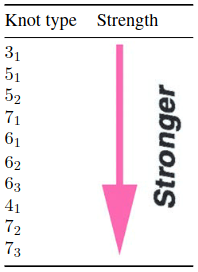
\includegraphics[scale=0.4]{str.png} }}%
    \qquad
    \subfloat[\centering узлы]{{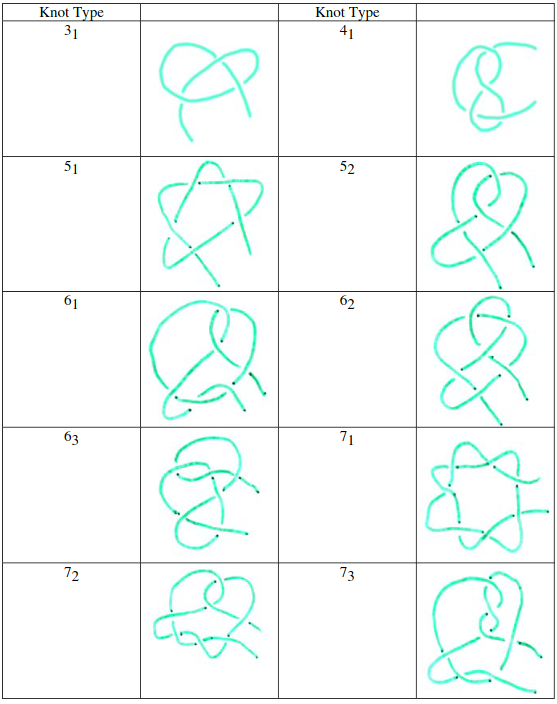
\includegraphics[scale=0.28]{type.png} }}%
    \caption{2 Figures side by side}%
    \label{fig:example}%
\end{figure}

\end{frame}

\begin{frame}
\frametitle{От самого прочного}

\begin{figure}%
    \centering
    \subfloat[\centering ранжирование]{{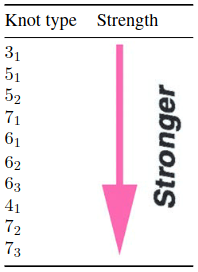
\includegraphics[scale=0.4]{str.png} }}%
    \qquad
    \begin{tabular}{ c c c }
    node 1 & force, kg \\
    $3_1$ & 7.6 \\
    $7_1$ & 7.5 \\
    $4_1$ & 8.1 \\
    $0$ & 10.4 \\
    \end{tabular}
\end{figure}

\end{frame}

\begin{frame}
\frametitle{От самого прочного}

\begin{figure}%
    \centering
    \subfloat[\centering ранжирование]{{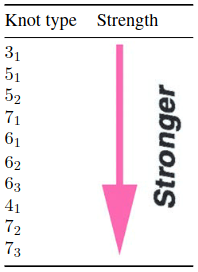
\includegraphics[scale=0.4]{str.png} }}%
    \qquad
    \begin{tabular}{ c c c }
    node 2 & force, kg \\
    $3_1$ & 6.8 \\
    $7_1$ & 8.0 \\
    $4_1$ & 8.2 \\
    $0$ & 12 \\
    \end{tabular}
\end{figure}

\end{frame}


\section{В процентах}

\begin{frame}
\frametitle{В процентах}

\begin{figure}%
    \centering
    \subfloat[\centering нить 1]{{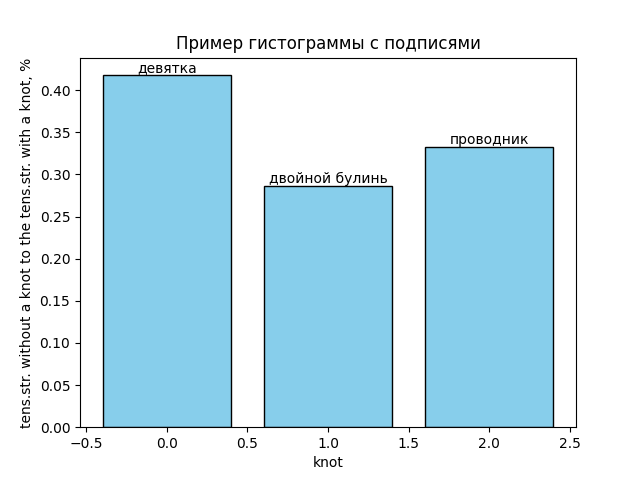
\includegraphics[scale=0.33]{data_1_thread_max_to_node.png} }}%
    \qquad
    \subfloat[\centering нить 2]{{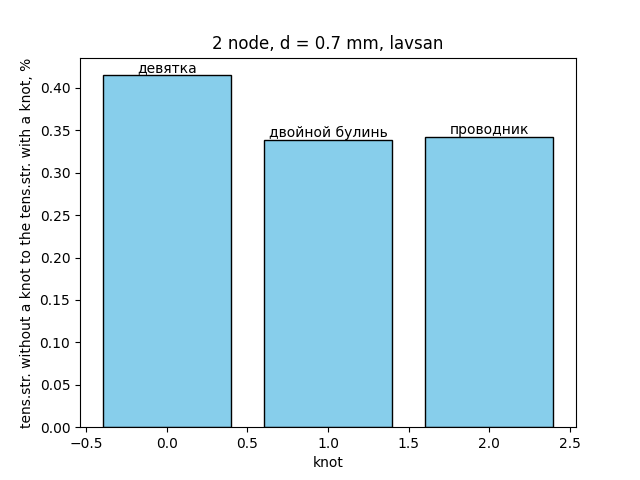
\includegraphics[scale=0.33]{data_2_thread_max_to_node.png} }}%
\end{figure}

\end{frame}


\end{document}
